\section*{Homework 3}

\setcounter{exercise}{0}

\begin{exercise}
Let \(\symcal{L}\) and \(\symcal{L}'\) be two lattices and let \(\varphi \colon \symcal{L} \to \symcal{L}'\) be an order-reversing bijection, with inverse \(\varphi^{-1}\).

\begin{enumerate}[(i)]
    \item Is \(\varphi^{-1}\) order-reversing?
    \item If \(\varphi\) and \(\varphi^{-1}\) are both order-reversing, prove that
    \begin{align*}
        \varphi(a \wedge b) = \varphi(a) \vee \varphi(b) \\
        \varphi(a \vee b) = \varphi(a) \wedge \varphi(b)
    \end{align*}
    for all \(a, b \in \symcal{L}\).
\end{enumerate}
\end{exercise}
\begin{solution}
\begin{enumerate}[(i)]
    \item The map \(\varphi^{-1}\) is not necessarily order-reversing, since it might not even be order-reflecting: \(a' \leq b'\) doesn't necessarily imply that \(\varphi^{-1} (a')\) can be compared with \(\varphi^{-1}(b')\).
    
    For an example, consider the order-reversing bijection \(\varphi\) between the following two lattices:
    \[
        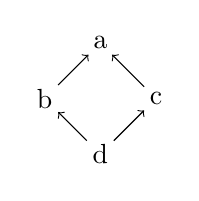
\begin{tikzpicture}[baseline=(current bounding box.center)]
            \node (top) at (0, 0) {a};
            \node[below left of = top] (left) {b};
            \node[below right of = top] (right) {c};
            \node[below right of = left] (bottom) {d};
            \draw[->, shorten <=-2pt, shorten >=-2pt,] (left) -- (top);
            \draw[->, shorten <=-2pt, shorten >=-2pt,] (right) -- (top);
            \draw[->, shorten <=-2pt, shorten >=-2pt,] (bottom) -- (left);
            \draw[->, shorten <=-2pt, shorten >=-2pt,] (bottom) -- (right);
        \end{tikzpicture}
        \xrightarrow{\varphi}
        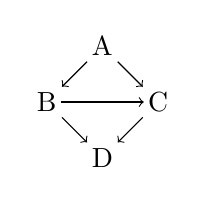
\begin{tikzpicture}[baseline=(current bounding box.center)]
            \node (top) at (0, 0) {A};
            \node[below left of = top] (left) {B};
            \node[below right of = top] (right) {C};
            \node[below right of = left] (bottom) {D};
            \draw[->, shorten <=-2pt, shorten >=-2pt,] (top) -- (left);
            \draw[->, shorten <=-2pt, shorten >=-2pt,] (top) -- (right);
            \draw[->, shorten <=-2pt, shorten >=-2pt,] (left) -- (bottom);
            \draw[->, shorten <=-2pt, shorten >=-2pt,] (right) -- (bottom);
            \draw[->, shorten <=-2pt, shorten >=-2pt,] (left) -- (right);
        \end{tikzpicture}
    \]
    If \(\varphi^{-1}\) were order-reversing, then \(X \leq Y\) would imply that \(\varphi^{-1}(X) \geq \varphi^{-1}(Y)\), for any \(X\) and \(Y\) in the second lattice. But while we have \(B \leq C\), their preimages \(\varphi^{-1}(B) = b\) and \(\varphi^{-1}(C) = c\) are in no relation in the first lattice.

    \item Let \(a, b \in \symcal{L}\). Let \(x \coloneq a \wedge b\). By the definition of the meet, we have that \(x \leq a\), \(x \leq b\) and for any \(c \in \symcal{L}\) with \(c \leq a\), \(c \leq b\) we must have \(c \leq x\).

    Since \(\varphi\) is order-reversing, we get that \(\varphi(x) \geq \varphi(a)\) and \(\varphi(x) \geq \varphi(b)\). For any \(c' \in \symcal{L}'\) with \(c' \geq \varphi(a)\) and \(c' \geq \varphi(b)\), we have that \(\varphi^{-1} (c') \leq \varphi^{-1}(\varphi(a)) = a\) and \(\varphi^{-1} (c') \leq \varphi^{-1}(\varphi(b)) = b\). Hence, since \(x\) is the meet of \(a\) and \(b\), we can deduce that \(\varphi^{-1} (c') \leq x\). Applying \(\varphi\) gives us \(\varphi(\varphi^{-1}(c')) = c' \leq \varphi(x)\), proving that \(\varphi(x) = \varphi(a \wedge b)\) is the join of \(\varphi(a)\) and \(\varphi(b)\), i.e. \(\varphi(a \wedge b) = \varphi(a) \vee \varphi(b)\).
\end{enumerate}
\end{solution}

\begin{exercise}
Let \(G\) be a group and \(E\) a field. A \emph{linear character} of \(G\) in \(E\) is a group homomorphism \(\sigma \colon G \to \symrm{GL}_1 (E)\).

Show that every set \(\Set{ \sigma_1, \dots, \sigma_n }\) of distinct linear characters of a group \(G\) in a field \(E\) is independent: if \(\sum_{i=1}^{n} x_i \sigma_i(g) = 0\) for all \(g \in G\), then \(x_i = 0\), \(\forall i = \overline{1, n}\). (i.e. \(\Maps{G}{E}\) is an \(E\)-vector space and \(\Set{ \sigma_1, \dots, \sigma_n } \subset \Maps{G}{E}\) is linearly independent)
\end{exercise}
\begin{proof}
We will prove this by induction.

For \(n = 1\), it's clear: \(x_1 \sigma_1 (g) = 0\) for all \(g \in G\) implies that \(x_1 = 0\), since \(\sigma_1 (g)\) is a unit in \(E\).

Suppose now that we know the statement holds for \(k - 1\) and want to prove it for \(k\). Let \(\Set{ \sigma_1, \dots, \sigma_k }\) be a set of independent linear characters and \(\Set{ x_1, \dots, x_k } \subset E\) such that
\[
    x_1 \sigma_1 (g) + \dots + x_k \sigma_k (g) = 0
\]
for all \(g \in G\).

Fix an element \(h \in G\). Multiplying the above equation by \(\sigma_{k} (h)\) gives
\[
    x_1 \sigma_1 (g) \sigma_k (h) + \dots + x_k \sigma_k (g) \sigma_k (h) = 0
\]
while replacing \(g\) with \(g h\) in the first equation gives
\begin{gather*}
    x_1 \sigma_1 (g h) + \dots + x_k \sigma_k (g h) = 0 \\
    \iff x_1 \sigma_1 (g) \sigma_1 (h) + \dots + x_k \sigma_k (g) \sigma_k (h) = 0
\end{gather*}
for all \(g \in G\). Subtracting the two new equations, the last term cancels out and we're left with
\[
    x_1 \cdot (\sigma_1 (h) - \sigma_k (h)) \cdot \sigma_1 (g) + \dots + x_{k - 1} \cdot (\sigma_{k - 1} (h) - \sigma_k(h)) \cdot \sigma_{k - 1} (g) = 0
\]
which holds for all \(g \in G\). More concisely,
\[
    \sum_{i = 1}^{k - 1} \left(x_i \cdot (\sigma_i (h) - \sigma_k (h))\right) \cdot \sigma_i = 0
\]
This is a linear combination of \(k - 1\) characters, so we can apply the induction hypothesis to conclude that the coefficients \(x_i \cdot (\sigma_i (h) - \sigma_k(h)) = 0\), for all \(i = \overline{1, k - 1}\). In particular, since the characters are \emph{distinct}, for each index \(i\) we can find some \(h_i \in G\) for which \(\sigma_{i} (h_i) \neq \sigma_{k} (h_i)\), which shows that \(x_i\) must be zero.

Replacing \(x_1 = \dots = x_{k - 1} = 0\) in the original equation, we have
\[
    x_k \sigma_k (g) = 0
\]
for all \(g \in G\). By the base case of the induction, \(x_k\) is also zero. Hence, \(x_i = 0\) for all \(i = \overline{1, k}\), which is what we had to show.
\end{proof}

\begin{exercise}
Let \(p\) be a prime number and \(n \in \naturals^*\). For \(q \coloneq p^n\), show that the finite field \(\finitefield{q}\) has exactly one subfield of order \(p^d\) for every divisor \(d\) of \(n\), and no others.
\end{exercise}
\begin{proof}
In the previous homework, we have shown that \(\Gal{\finitefield{q}}{\finitefield{p}}\) is cyclic of order \(n\). We will denote this group by \(C_n\).

Using the Galois correspondence, the conclusion is equivalent to showing that \(C_n\) has exactly one subgroup of index \(d\). Letting \(e = n / d\), this is the same as showing that \(C_n\) has exactly one subgroup of order \(e\).

The basic theory of cyclic groups tells us that \(C_n\) is isomorphic to \(\left(\integersmod{n}, +\right)\). The subgroup generated by \(\widehat{d}\) is \(\Set{ \widehat{0}, \widehat{d}, 2 \widehat{d}, \dots, (e-1) \widehat{d} }\), which has order \(e\). Conversely, if \(\Set{ \widehat{0}, \widehat{x_1}, \dots, \widehat{x_{e - 1}} }\) is a subgroup of order \(e\), then we can write each element \(\widehat{x_j}\) as \(k_j \, \widehat{1}\). Furthermore, we have \(e \, \widehat{x_j} = \widehat{0}\) for any \(j\), since the order of any individual element must divide the order of the subgroup. Combining these two remarks shows us that \(e k_j \widehat{1} = \widehat{0}\), hence \(e \cdot k_j = n \cdot m\) for some \(m \in \naturals\). Writing \(n = d \cdot e\), we get that \(k_j = d \cdot m\), hence this subgroup is actually the one generated by \(\widehat{d}\).
\end{proof}
